\documentclass[a4paper, fontsize=12pt]{scrartcl}
\usepackage{cmap}
\usepackage[left=2cm,right=2cm,top=2cm,bottom=2cm]{geometry}
\usepackage{indentfirst}
\usepackage{setspace}
\textheight=24cm % высота текста
\setlength{\parindent}{1cm}
\usepackage[]{cite}
\usepackage[T2A]{fontenc}
\usepackage[utf8]{inputenc}
\usepackage[english, russian]{babel}
\usepackage{amsmath, amsfonts, amssymb, amsthm}
\usepackage{graphicx, epsfig}
\graphicspath{{pictures/}}
\DeclareGraphicsExtensions{.pdf,.png,.jpg}
\usepackage{subfig}
\usepackage{color}
\usepackage{gensymb}
\usepackage{enumitem}	
\setlist{nolistsep} 
\usepackage{algorithm}
\usepackage{algpseudocode}
\floatname{algorithm}{Алгоритм}
\algnewcommand{\IIf}[1]{\State\algorithmicif\ #1\ \algorithmicthen}
\algnewcommand{\EndIIf}{\unskip\ \algorithmicend\ \algorithmicif}
\renewcommand{\algorithmicend}{\textbf{завершим}}
\renewcommand{\algorithmicif}{\textbf{если}}
\renewcommand{\algorithmicelse}{\textbf{иначе}}
\renewcommand{\algorithmicthen}{\textbf{то}}
\renewcommand{\algorithmicdo}{\textbf{выполним}}
\renewcommand{\algorithmicfor}{\textbf{цикл для}}
\renewcommand{\algorithmicforall}{\textbf{цикл для всех}}
\renewcommand{\algorithmicwhile}{\textbf{цикл пока}}
\usepackage{hyperref}
\usepackage [section] {placeins}


\begin{document}

\begin{raggedright}
Желаемые секции: «Разработка компонент модели системы Земля», «Процессы на поверхности суши: наблюдения, модели и усвоение данных»
\end{raggedright}


\begin{center}
    \Large
    \textbf{\textsc{Модификация почвенно-снежного блока климатической модели ИВМ РАН}}
    \normalsize 
    
    \textbf{\textit{Черненков Алексей Юрьевич$^{1, *}$, Кострыкин Сергей Владимирович$^{2-4, **}$, Володин Евгений Михайлович$^{2, ***}$}}
    
            $^1$Московский физико-технический институт (национальный исследовательский университет), Институтский переулок, д. 9, Долгопрудный, Московская область, 141701 Россия
    
            $^2$Институт вычислительной математики им. Г.И. Марчука РАН, ул. Губкина, д. 8, Москва, 119333 Россия
    
            $^3$Институт глобального климата и экологии им. Ю.А. Израэля, ул. Глебовская, д. 20Б, Москва, 107258 Россия
    
            $^4$Институт физики атмосферы им. А.М.Обухова РАН, Пыжевский пер., 3, Москва, 119017 Россия
    
            $^*$e-mail: \url{chernenkov.ayu@phystech.edu}
    
            $^{**}$e-mail: \url{s_kostr@mail.ru}
            
            $^{***}$e-mail: \url{volodinev@gmail.com}
    
\end{center}







\section{Введение}

В последние десятилетия активно развивается моделирование климата. Для корректного описания круговорота воды важно, чтобы модели правильно обрабатывали сезонный снежный покров.

В переходные сезоны, когда температура колеблется около нулевой отметки, снег может таять, но при этом на верхнюю границу почвы уходит не вся талая вода, некоторая ее часть задерживается в слое и может перезамерзать. Также с течением времени после снегопада снежные частицы сминаются и слипаются, в результате чего снег уплотняется. Все эти факторы влияют на свойства снежного покрова. 

В данной работе рассматривается пятая версия климатической модели ИВМ РАН (INMCM5). Данная модель состоит из двух основных блоков: модели общей циркуляции атмосферы и модели общей циркуляции океана. Данная версия модели участвует в международном проекте по сравнению климатических моделей CMIP6 (Coupled Models Intercomparison Project). Некоторые результаты по моделированию современного климата с помощью данной модели представлены в работе \cite{Volodin2017}.

В работе описываются изменения в описании снега моделью. Модифицируется процесс таяния, а также реализуются процесс перезамерзания талой воды и изменение плотности снежного покрова, которая ранее считалась постоянной: $\rho_{snow} = 0.1854 $ г/cм$^3$. Стоит отметить, что изменения затрагивают только атмосферный блок.


\section{Описание внесенных изменений в модель}

Изменения в описании снега затрагивают почвенно-снежный блок, который входит в атмосферную часть модели. Данный блок представлен одномерной моделью, описывающей процессы тепло- и влагопереноса в почве, растительности и снежном покрове, а также обмен этой системы теплом и влагой с атмосферой, его описание достаточно подробно приведено в работах \cite{Volodin1998, Volodina2000}.  

Определим переменные, необходимые для описания внесенных изменений: 
\begin{itemize}
    \item $S$ -- водно-эквивалентная толщина слоя снега,
    \item $S_{sn}$ -- "настоящий"\  снег (по сути, крошка из пористого льда), 
    \item $M_{soil}$ -- вода, поступившая на поверхность почвы,
    \item $P$ -- интенсивность осадков при температуре подстилающей поверхности, меньшей $0 ~\degree$C,
    \item $\lambda$ -- удельная теплота плавления льда, 
    \item $\mathcal{L}$ -- удельная теплота парообразования, 
    \item $\mathcal{E}$ -- поток скрытого тепла на поверхность снега, идущего на испарение/сублимацию,
    \item $\rho_w$ -- плотность воды,
    \item $M$ -- интенсивность снеготаяния,
    \item $S_{wat}$ -- талая вода, оставшаяся в слое снега,
    \item $F$ -- интенсивность замерзания воды,
    \item $S_{rfrz}$ -- перезамерзшая талая вода (по сути, крошка из плотного льда),
    \item $T_{sn}$ -- температура снега, 
    \item $\Delta E$ -- избыточный/дефицитный поток тепла в тепловом балансе на поверхности.
\end{itemize}

В исходной версии модели водно-эквивалентная толщина слоя снега вычисляется на основании следующего уравнения баланса:
\begin{equation}
    \dfrac{\partial S}{\partial t} = P - M - \dfrac{\mathcal{E}}{\mathcal{L} \cdot \rho_w}  \label{sys}
\end{equation}
Процесс таяния начинается, когда температура подстилающей поверхности становится больше $0 ~\degree$C, при этом весь растаявший снег, а также возможный дождь, выпавший при наличии снежного покрова, поступают на поверхность почвы.

Идея модификации заключается в более физичном описании процесса снеготаяния. Предполагается, что при таянии снега вода не уходит моментально на верхнюю границу почвы, а постепенно просачивается сквозь толщу снега. При этом талая вода может замерзать, отдавая тепло снежному покрову. Стоит отметить, что теперь снежный покров представляется как некоторая субстанция, состоящая из трех фракций: непосредственно снега в обычном представлении, талой вода, содержащейся в нем и перезамерзшего снега. 

Процесс снеготаяния--перезамерзания реализуется с помощью \textbf{Алгоритма \ref{alg:setup}}. 
Критическая масса воды $S_{wat}^{max}$, способная содержаться в слое снега зависит от количества снега и его пористости $\varepsilon_{sn}$. Предлагается оценивать эту массу \cite{Gusev2002} и пористость снега \cite{Stock} по следующим формулам:
\begin{equation}
     S_{wat}^{max} = S ~\dfrac{\varepsilon_{sn}}{1 - \varepsilon_{sn}}  \label{sys}  
\end{equation}
\begin{equation}
    \varepsilon_{sn} = 0.11 \left( \dfrac{\rho_w}{\rho_{sn}} - 1 \right)  \label{sys}  
\end{equation}

\begin{algorithm}[H]
\caption{Процессы таяния снега и перезамерзания талой воды}
\label{alg:setup}
\begin{algorithmic}[]
    \If{$ \Delta E >0$, $T_{sn} = 0 ~\degree$C и $S^{n-1} > 0 $}
        \State $ M = \dfrac{\Delta E}{\lambda} $, ~ $ \delta = \dfrac{S_{sn}^{n-1}}{S_{sn}^{n-1} + S_{rfrz}^{n - 1}}$ 
        \State $ S_{sn}^n = S_{sn}^{n-1} + P - \Delta t \left( \dfrac{\mathcal{E}}{\mathcal{L} \cdot \rho_w} + \delta \cdot M \right) $ 
        \State $ S_{rfrz}^n = S_{rfrz}^{n - 1} - \Delta t (1 - \delta)M $ 
        \State $ S_{wat}^{max} = f( S_{sn}^n ) $, ~ $ \Delta S_{wat} = max\{\Delta t \cdot M, ~S_{wat}^{max}\} $ 
        \State $ M_{soil} = max\{\Delta t \cdot M - S_{wat}^{max}, ~0\} $ 
        \State $ S_{wat}^n = S_{wat}^{n-1} + \Delta S_{wat} $ 
    \Else
        \If{$S^{n-1} > 0$, $S_{wat}^{n-1} > 0$ и $T_{sn} = 0 ~\degree$C}
            \State $F = -\dfrac{\Delta E}{\lambda}$, ~ $S_{sn}^n = S_{sn}^{n-1} + P - \Delta t \left( \dfrac{\mathcal{E}}{\mathcal{L} \cdot \rho_w} - F \right)$
            \State $S_{rfrz}^n = S_{rfrz}^{n - 1} + ( S_{wat}^{n-1} - S_{wat}^n )$
            \State $S_{wat}^n = max\{ S_{wat}^{n-1} - \Delta t \cdot F, ~0\}$
        \EndIf
    \EndIf
    \State $S^n = S_{sn}^n + S_{wat}^n + S_{rfrz}^n$
\end{algorithmic}
\end{algorithm}



Эволюцию плотности снега предлагается описывать как в модели SWAP \cite{Gusev2002, Yosida1955}:
\begin{equation}
    \rho_{sn}(\tau_i) = \rho_{sn}(\tau_{i-1}) \left[  1 + 0.1 H_{sn}(\tau_{i-1}) \exp \{ 0.08 T_{sn} - 21 \rho_{sn}(\tau_{i-1})  \} \right]    \label{sysRHOOLD}  
\end{equation}
В данной модели $H_{sn}$ -- водно-эквивалентная толщина слоя снега в сантиметрах, плотность снега $\rho_{sn}$ вычисляется в г/см$^3$, температура слоя снега $T_{sn}$ задается в градусах Цельсия. Нужно заметить, что здесь шаг по времени 1 сутки, поэтому для использования данной зависимости в модели ИВМ была необходима переинтерполяция. Чтобы учесть все фракции снега, предлагается рассчитывать плотность снежного слоя как среднее взвешенное:
\begin{equation}
    \rho_{snow} = \rho_{old} \cdot \delta_{old} + \rho_{new} \cdot \delta_{new} + \rho_{w} \cdot \delta_{wat} + \rho_{ice} \cdot \delta_{rfrz}
\end{equation}
Здесь $\rho_{old}$ -- плотность лежалого снега, рассчитанная по эволюционной модели,  $\rho_{new} = 0.1$ г/см$^3$ -- плотность свежевыпавшего снега, $\rho_{w} = 1$ г/см$^3$ -- плотность воды, $\rho_{ice} = 0.917$ г/см$^3$ -- плотность льда, $\delta_{old}, ~\delta_{new}, ~\delta_{rfrz}, ~ \delta_{wat}$  -- массовые доли (в водном эквиваленте) старого, свежего, перезамерзшего снега и талой воды.




\section{Результаты}
Для тестирования внесенных изменений были проведены расчеты климата в 1997--2002 годах с исходной и модифицированной версиями модели. Из результатов расчетов следует, что внесенные изменения в почвенно-снежный блок, приводят к более позднему сходу снега (в отдельных регионах разница доходит до месяца), а процесс формирования снежного покрова происходит более интенсивно. Так, теперь в Заполярье, горах на западном побережье Канады и Аляски, а также в районе Гималаев в некоторых районах снег продолжает сохраняться даже в июне, в то время как раньше он практически весь успевал стаять в течении мая. Вклад описанных процессов в формирование устойчивого снежного покрова в конце осени -- начале зимы наиболее заметен в заполярных регионах Евразии и Гималаях. Эти результаты согласуется с архивными данными наблюдений за климатом, например, данные National Centers for Environmental Information (NCEI). Также можно отметить хорошее согласие по моментам образования и схода снежного покрова и территориям, на которых он лежит, с данным Глобального реанализа CAMS (EAC4) Европейского центра среднесрочных прогнозов погоды. 

Также нужно отметить, что более подробное описание почвенно- снежного блока привело к увеличению количества снега в целом. Наибольшее различие между версиями наблюдается в весенние месяцы, при этом с июля по сентябрь различия минимальны. В сравнении с данными наблюдений и реанализа суммарная масса снега в случае модифицированной версии оказывается завышенной, но, вместе с тем, описание площади, покрытой снегом, наоборот, улучшается. Заметим, полученные результаты согласуется с тенденцией к завышению массы снега при более точном описании площади покрытия в ряде климатических моделей, участвующих в CMIP6, при использовании более подробного описания снега \cite{Mudryk}.

\begin{figure}[h]
    \begin{minipage}[h]{0.49\linewidth}
        \center{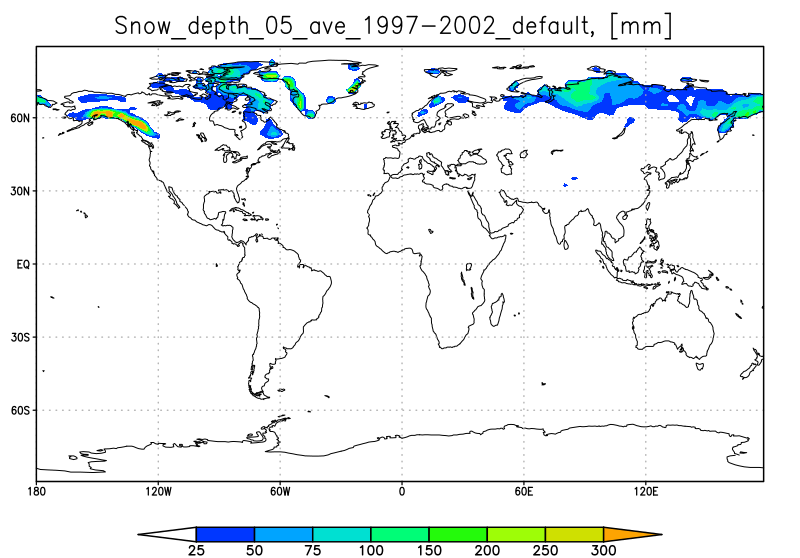
\includegraphics[width=1.1\linewidth]{Snow_depth_05_ave_1997-2002_default.png} \\ (а)}
    \end{minipage}
    \hfill
    \begin{minipage}[h]{0.49\linewidth}
        \center{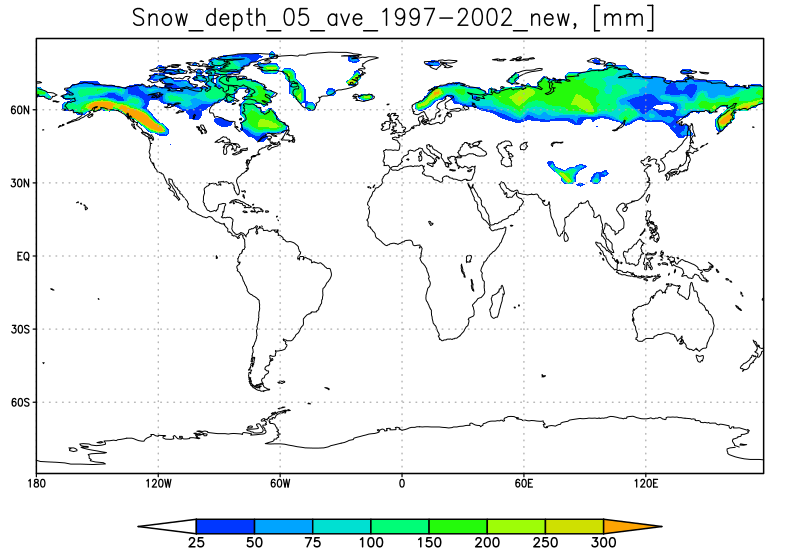
\includegraphics[width=1.1\linewidth]{Snow_depth_05_ave_1997-2002_new.png} \\ (б)}
    \end{minipage}
    \caption{Среднемесячная водно-эквивалентная толщина слоя снега по данным (а) исходной и (б) модифицированной версий модели ИВМ (месяц -- май) }
    \label{fig:image}
\end{figure}


\section{Заключение}

В ходе данной работы был модифицирован почвенно-снежный блок глобальной климатической модели ИВМ РАН, в результате чего было улучшено воспроизведение площади поверхности, покрытой снегом, в сравнении с данными реанализа. В модифицированной версии снег разделяется на лежалый, свежевыпавший и перезамерзший, а также учитывается талая вода, которая может содержаться в слое снега. Стоит отметить,  что полученный результат можно использовать для подробного описания метаморфизма снега и более точного расчета снежного альбедо. 



\begin{thebibliography}{9}

\bibitem{Volodin2017} 
Volodin, Evgeny and Mortikov, Evgeny and Kostrykin, Sergey and Galin, V. and Lykossov, Vasily and Gritsun, Andrey and Diansky, Nikolay and Gusev, Anatoly and Iakovlev, Nikolay. Simulation of the present-day climate with the climate model INMCM5. Climate Dynamics, 2017, Vol. 49, DOI: 10.1007/s00382-017-3539-7.

\bibitem{Volodin1998} Володин, Лыкосов,  Параметризация процессов тепло- и влагообменав системе растительность–почва для моделирования общей циркуляции атмосферы. Описание и расчеты с использованием локальныхданных наблюдений, Известия РАН. Физика атмосферы и океана., 1998, No 4., С. 453–465.

\bibitem{Volodina2000} Володина, Бенгтссон, Лыкосов, Параметризация процессов тепло-влагопереноса в снежном покрове для моделирования сезонных вариаций гидрологического цикла суши, Метеорология и гидрология., 2000, Т. 10, No 5. 

\bibitem{Gusev2002} 
Gusev Y. M., Nasonova O. N., The simulation of heat and water exchange at the land–atmosphere interface for the boreal grassland by the land-surface model SWAP, Hydrological Processes., 2002, Vol. 16, no. 10, P. 1893–-1919.

\bibitem{Stock} 
Кучмент, Демидов, Мотовилов, Формирование речного стока. Физико-математические модели, Под ред. С. В. Музылева., Наука, Москва, 1983, Т. 216.

\bibitem{Yosida1955} 
Yosida Z. et al, Physical studies on deposited snow. Thermal properties., Contributions from the Institute of Low Temperature Science., 1955, Vol. 7, P. 19–74.

\bibitem{Mudryk} 
L. Mudryk, M. Santolaria-Otin, G. Krinner et al, Historical Northern hemisphere snow cover trends and projected changes in the CMIP6  multi-model  ensemble, The Cryosphere, 2020, Vol. 14, No. 7, P. 2495–2514.

\end{thebibliography}

\newpage

\begin{center}
    \Large
    \textbf{\textsc{Modification of the soil-snow block of the climatic model of the INM RAS}}
    \normalsize 
    
    \textbf{\textit{Chernenkov Alexey Yurievich$^{1, *}$, Kostrykin Sergey Vladimirovich$^{2-4, **}$, Volodin Evgeny Mikhailovich$^{2, ***}$}}
    
            $^1$Moscow Institute of Physics and Technology, Moscow Region, Dolgoprudny, 141701 Russia
    
            $^2$Marchuk Institute of Numerical Mathematics, Russian Academy of Sciences, Moscow, 119333 Russia
    
            $^3$ Izrael Institute of Global Climate and Ecology, Moscow, 107258 Russia
    
            $^4$Obukhov Institute of Atmospheric Physics, Russian Academy of Sciences, Moscow, 119017 Russia
    
            $^*$e-mail: \url{chernenkov.ayu@phystech.edu}
    
            $^{**}$e-mail: \url{s_kostr@mail.ru}
            
            $^{***}$e-mail: \url{volodinev@gmail.com}

\end{center}

Climate modeling has been actively developing in recent decades. To  describe the water cycle correctly, it is important that the models describe the seasonal snow cover correctly.

During the transitional seasons, when the temperature fluctuates around zero point, the snow can melt, but part of the melt water stays inside the layer and can refreeze. Also, some time after the snowfall, the snow becomes denser. All these affect the properties of the snow cover.

This paper considers the fifth version of the climate model of the INM RAS (INMCM5). Here described the changes in the soil-snow block of the model: changes of melting process and density of the snow cover,  implementation of the process of refreezing of melt water.

It is assumed that when the snow melts, the water does not immediately go to the upper boundary of the soil, but seeps through the thickness of the snow. In this case, the melt water can refreeze, giving off heat to the snow cover. It is worth noting that now the snow cover is presented as a certain substance, consisting of three evenly mixed fractions: snow in the usual view, melt water contained in it, and refrozen snow. The evolution of the snow density is described as in the SWAP model. To take into account all fractions of snow, it is proposed to calculate the density of the snow layer as weighted average.

To test the changes made, climate calculations were carried out in 1997--2002 with the original and modified versions of the model. It follows from the calculation results that the changes into the soil-snow block lead to a later melting of snow, and the process of snow cover formation has become more intensive. This is especially noticeable in the Arctic, on the western coast of Canada and Alaska, as well as in the Himalayas. It can be noted good according to the data of the formation and disappearance of snow cover and the territories on which it lies with the data of the CAMS Global Reanalysis (EAC4) of the European Centre for Medium-Range Weather Forecasts and observation data.

Note that the result obtained can be used for a detailed description of snow metamorphism and a more accurate calculation of the snow albedo.


\end{document}
